\documentclass{article}
\usepackage[utf8]{inputenc}
\usepackage{hyperref}
\usepackage{float}
\usepackage[table,xcdraw]{xcolor}
%\usepackage[sort&compress,square,comma,authoryear]{natbib}
\usepackage{booktabs}
\usepackage{graphicx}
\graphicspath{{Figures/}}
\usepackage{longtable}

\usepackage[
backend=biber,
style=authoryear,
sorting=nyt % sort by name year title
]{biblatex}
\addbibresource{Ref_invertebrate_DB.bib}

\title{ OUTLINE: Harmonized macroinvertebrate trait database, Aggregation of traits, Trait definitions, Sources }
\author{}%Stefan Kunz 
\date{}%June 2019


\begin{document}
%TODO: Use citep & citet instead of cite
\maketitle

\section{Introduction}

% !General introduction: Invertebrates importance/biodiversity and stressor
% ? use Traits mechanistic relationship, environmental filtering
% Half of all described freshwater invertebrates are aquatic insects

In the age of the Anthropocene invertebrates are exposed to multiple stressors such 
as chemical pollution, hydro-morphological modifications, invasive species and climate change. %?Sources 
Freshwater invertebrates play a crucial role for many ecosystem processes such as 
carbon cycling and water purification. In addition to their functional role, 10 \% of all 
described species live in freshwaters, most of which being invertebrates, and thus represent a
large part of animal biodiversity.
Understanding distributions of invertebrate communities and predicting effects of 
potential stressors is a long time goal of freshwater research. Since the 1970s 
ecologists have started using organismal traits to group aquatic insect species % ?to understand what -> Check Cummins

Traits are biological characteristics or ecological preferences measurable at the 
individual organism. %? Source Lancaster? Find precises definition
They reflect an organisms adaptation to its habitat. Trait based approaches in 
ecology are based on the habitat template theory, that predicts where environmental conditions
are similar trait composition should also converge, even across biogeographic boundaries. %?Source
Furthermore, several studies suggested that trait variability is lesser on larger geographical
scales than taxonomic variability. %?Source Bonada 
Hence, trait based approaches can be a suitable tool for comparing the effect of various 
environmental stressors to invertebrate communities on large scales or across regions. 
%!General studies? Or more specific to studies for several regions
% They have been used to understand species distributions, in predicting effects of various environmental
% stressors to invertebrate communities, and as tool in biomonitoring. %? Source: Statzner & Beche 2010, Ralf Paper, Cummins Paper?
Consequently, studies have been carried out that e.g. examine the relationship between climate
and freshwater community assemblages using species traits. % TODO: Cite Bhowmik, cite Brown 
% TODO: Enrich with examples -> Maybe for toxicants as well?
Many of such studies combine information from several trait databases. For example, 
Brown et al. used in their study traits from invertebrate trait databases from
Europe, North America and New Zealand to investigate the effect of decreasing glacier cover
to river ecosystems. %TODO Cite Brown

% Studies that use information on aquatic invertebrate traits from different regions
% and/or aggregate trait information are increasing 
% !Transition into trait data
In fact, invertebrate trait data are increasingly available. Over the last decades aquatic 
ecologists have compiled comprehensive databases on invertebrate traits for different regions 
(see table \ref{tab:trait_databases} for examples). 
% !Mention various problems with trait databases 
However, researchers face various problems when they need to synthesize information from 
multiple invertebrate trait databases. 
% !Trait terminology
i) The use of inconsistent terminology across studies (see \cite{schmera_proposed_2015}
for a comprehensive discussion). 
For example, some studies used the term "trait" to describe a general 
organismal property like "generations per year" (\cite{statzner_reproductive_1997}, 
\cite{ussegliopolatera_biological_2000}), while in other studies this 
term was related to categories like "bi/multivoltine" 
(\cite{haybach_use_2004}, \cite{vieira_database_nodate}). Here, we follow 
the proposal of Schmera et al. (2015) and use the term \textit{trait} for a morphological,
physiological, or phenomenological feature measurable at the individual
organism (e.g. tegument, gills, etc.) and the term \textit{grouping feature} to describe 
a general property of related organismal traits (e.g. respiration). 
%? Include measurement scale?
%TODO: in concordance with previous paragraphs on trait definitions
%! Different traits used/definitions
ii) Invertebrate trait databases from different regions are not standardized. 
Often, the same grouping features are categorized using different traits. 
% TODO Example
This is complicated by the use of different measurement scales. For example, trait databases 
from North America use traditionally a binary coding (i.e. trait is expressed or not), 
whereas most other trait databases (e.g. Tachet, freshwaterecology, and New Zealand) 
use fuzzy coding (i.e. trait is expressed to a certain extent by the organism). 
Hence, transformation of nominal scale to ratio scale or vice versa is required. %? Wording
Furthermore, definitions for some traits differ as well across databases. 
% TODO Example feeding!
%! Taxonomical resolution & traits aggregation -> no guidance
%! Wording: taxonomical resolution -> high -> species level 
% high taxonomical level -> high -> genus/family,...(Schmidt-Kloiber et al.)
iii) Taxonomical resolution between databases differs, further complicating the
synthesis of trait data from different regions. Some trait databases have recorded
information on mixed levels of taxonomical resolution like the North American trait
database or the Australian trait database. In contrast, trait information in the 
freshwaterecology database is entirely recorded on species-level. %?ref to graphic
%TODO: Percentages of different levels of taxonomical resolutions in process overview graph 
Using trait information on varying taxonomical levels is only possible when 
traits are aggregated to the lowest taxonomical level that is shared by all used databases. 
However, iv) so far studies comparing different ways of aggregating traits are lacking.
% Hence, guidance on how to perform a robust trait aggregation is missing. 
% TODO Poff Paper example, check Brown and other literature

%!Incentive of our analysis:
% no API/R packages 
Given the problems mentioned above extensive data processing is required before researchers 
can use multiple invertebrate trait databases for their work. 
In this paper we examine difficulties that ecologists face when synthesizing trait 
information from different invertebrate trait databases. We explore the effect of different
decisions researches have to make when working with invertebrate trait data 
from several sources, involving trait harmonization, handling different codings,
normalization, and aggregation of traits.
%?Effect of a statistical analysis -> Clustering?
%!What we did/Goal:
Therefore, we harmonized six grouping features of different trait databases from four
regions and aggregated the trait information to family-level. % ?Name Traits
We discuss the harmonization and show the effect of different ways of aggregating 
traits (inter alia Problem of different coding styles (fuzzy vs binary)).
We also present an overview of differences in trait definitions among databases.
Finally, our paper compares the references for the trait information that 
were specified in the trait databases we used.


%TODO: Change heading to be more expressive
\section{Methods}

\subsection{Description of harmonized trait databases} 

% TODO Give a motivation (better in introduction?)
The harmonized databases are using the available information on aquatic invertebrate
traits for the regions Europe, North America, Australia, and New Zealand. 
Due to the different number and identity of grouping features in each database, 
the following six grouping features were chosen for this study: locomotion, feeding mode, 
respiration, voltinism, size, and body form. 
%? Next two sentences can be removed?
% Comment: For C of TPG Development pattern added
% TODO: Few words why these grouping features have been selected
% TODO: Reasoning why no ecological grouping features have been used
Trait information for Australia and New Zealand were retrieved from 
a single database, respectively. For Europe we gathered trait information from the 
freshwaterecology trait database (\url{https://www.freshwaterecology.info/}) 
and complemented where possible missing information with the 
Tachet trait database (\cite{usseglio-polatera_biomonitoring_2000}). 
North American invertebrate traits were retrieved from Laura Twardochleb and 
complemented where possible by trait information from Vieira et al (\cite{vieira_database_nodate}).
From now on, if we use the term European or North American trait database we refer to the combined 
databases unless explicitly stated otherwise.
We used all available information on invertebrates in the databases but restricted
our analysis to those taxa that have complete trait profiles for the grouping features
mentioned earlier. We are aware that imputation methods exist, which infer missing 
information for traits by interpolating from related traits. % TODO: Cite Penone
However, by using only complete data we were able to evaluate the taxonomical coverage
per order within the databases. We consider this a helpful information for researchers
who strive to fill data gaps.
Table \ref{tab:trait_databases} gives an overview of the used databases. 
In the following paragraphs, we describe the data processing steps required to 
establish a harmonized invertebrate trait database. 

\begin{table}[H]
    \centering
    \caption{Overview of trait databases.}
    \label{tab:trait_databases}
    \begin{tabular}{lll}
    \toprule
   Region & Coding of trait states & Reference \\ 
    \hline
   Europe & Largely fuzzy & \cite{schmidt-kloiber_www.freshwaterecology.info_2015}\\ 
   Central Europe & Fuzzy coded & \cite{usseglio-polatera_biomonitoring_2000} \\ 
   North America & Largely binary & \cite{vieira_database_nodate}\\
   North America & Largely binary & cite Laura Twardochleb \\
   Australia & Binary \& fuzzy coding  & \cite{kefford_ben_AST_DB_2019}\\ 
   New Zealand & Fuzzy coded & \\ %TODO: Create entry for more recent NZ reference
    \bottomrule
    \end{tabular}
\end{table}


\subsection{Normalization \& data conversion}

%TODO Mention taxonomical corrections?
% !Issues with coding & scale in the trait databases
Establishing a harmonized database required traits on the same measurement scale to 
enable comparability. However, in the used databases traits varied within and among databases 
in terms of measurement scale. Traits were either fuzzy coded, binary coded or 
to a small extent coded as continuous variable (e.g. size). Fuzzy codes capture the variation 
(i.e. temporal or spatial) in a trait and are represented by affinity scores 
(sometimes termed membership state) which express a preference of a taxon to a certain trait.
Usually, these scores range from 0 representing no affinity to an arbitrary maximum value which 
represents high affinity. This type of coding uses the ratio scale and not the ordinal
scale as one might intuitively assume. In fact, the intention of the developers of this 
coding system was to convert affinity scores to percentages per trait, e.g. 
for a grouping feature with four traits affinity scores of \textit{5, 6, 2, 2} are equal
to \textit{1/3, 2/5, 2/15, 2/15} or \textit{33.3 \%, 40 \%, 13.3 \%, 13.3 \%} (\cite{chevenet_francois_fuzzy_1994}).
We used fuzzy coded traits for establishing our harmonized databases where possible, otherwise binary traits. 
Categorical and continuous traits across all used databases were converted into binary traits. 
Implicitly, we assumed for binary variables that a value of 1 for a particular trait corresponded
to the maximum affinity of a taxon for that particular trait.

Two databases needed further data processing. Firstly, the Australian database which is a collection of seven trait databases. 
Thus, several grouping features occur multiple times but with traits that have different types of codings and ranges.
For example, body size occurs as continuous variable, with traits that are fuzzy coded, and with traits that are binary coded. 
The same traits originating from different sub-databases in the Australian trait database were allocated. 
To enable allocation of fuzzy coded and binary traits we applied a range normalization by dividing each fuzzy coded 
trait by its potential maximum value. Consequently, the values of each trait were converted to a range from 0 to 1.

Secondly, the North American trait database which only contained traits on the nominal scale. 
We first converted nominal traits into binary traits. As a second approach we converted nominal traits for taxa 
on species and genus-level into "pseudo" fuzzy codes by calculating the percentage of occurrence for each
trait per genera and grouping feature. Both approaches were compared regarding the trait values they yielded.
We refer to the version with binary traits as \textit{NOA\_bin} and to the version with pseudo fuzzy codes as 
\textit{NOA\_fuzzy}. 
% Better wording? traits from NOA data were converted to fuzzy codes by allocating at genus level using frequency on species level

% Furthermore, in some databases fuzzy coded information occurred in different ranges 
% (e.g. from 0 to 3 and from 0 to 5 in the Tachet database, from 0 to 10 in the 
% freshwaterecology database). 

% !Issue of duplicate taxa
The Australian, Tachet, and the North American trait databases contained duplicate taxa entries
- either on species, genus or family-level - which were amalgamated. 
The duplicate entries in the Australian trait database originated from the different sub-databases. 
As a result, many of the duplicate entries complemented each other (e.g. for a given trait one duplicate contained a value, 
the other not). In those cases where several different values for a trait occurred, the average trait value was calculated. 
The NOA\_bin database only contained 0 and 1 as entries. Hence, for duplicates the maximum value was taken.
% Tachet: Fuzzy codes -> Mean
For the tachet trait database duplicate entries were allocated using the mean if they contained contrasting
information on the same trait. 
% ?What about zero's -> were disregarded

% !Normalization/Standardization 
Finally, every trait within each grouping feature was standardized by the sum of all traits 
within this particular grouping feature per taxon to convert traits to percentages per trait. 
% which can be used to compare and harmonize taxa regarding their traits. %!Wording

\subsection{Harmonization of traits and taxa}
% TODO Differences in trait definitions
% TODO Sources of traits

% !What is harmonization? & Why is it needed?
Harmonization of traits means amalgamating several similar traits into a single trait. 
It has to be undertaken when grouping features from different sources (e.g. different regions) are
used and the grouping features do not contain the same traits. 
For example, in our study for the grouping feature locomotion the lowest number of traits that occur
across all databases was in the New Zealand trait database ("Swimmer", "Burrower", "Crawler", "Sessil"). 
Hence, in all other databases locomotion traits have been allocated into these four traits (see \ref{fig:harmon_overview_1}
and \ref{fig:harmon_overview_2}).
% !Taxonomical harmonization
% Harmonization is crucial -> number of cases & comparability
%?Give an example -> Clusteranalysis

% !How was the harmonization done? -> technical aspect.
Grouping features that differed in their traits among databases have been harmonised by condensing the traits in such a way
that in the end the same grouping features in all databases consisted of the same traits.  
Thereby, traits were amalgamated based on ecological knowledge or expert judgment. %!Wording 
Our approach of harmonizing the traits in the used databases is outlined in figures 
\ref{fig:harmon_overview_1} and \ref{fig:harmon_overview_2}. 

% TODO: Harmonization for feeding mode AUS needs to be finished!
\begin{figure}[H]
   \centering
   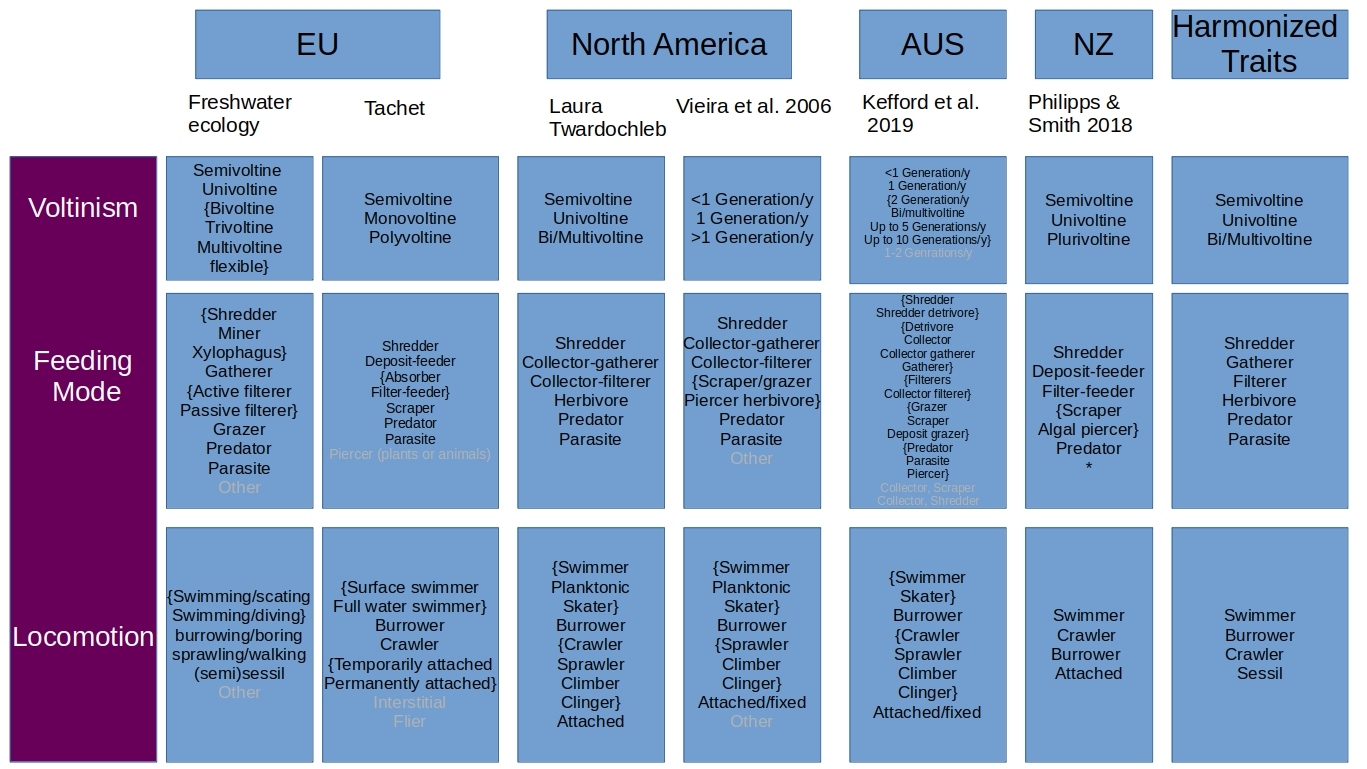
\includegraphics[width=16.5cm, height=10cm]{trait_overview1.jpg}
   \caption{Proposed harmonization scheme for the grouping features
   voltinism, feeding mode and locomotion. Shown are all traits for the 
   used grouping features in the investigated trait databases and 
   the harmonized traits in the end. Traits in curly brackets were 
   harmonized to one trait. Traits highlighted in Grey were omitted. \newline
   \textit{* Trait parasite was not available in New Zealand trait database.}
   }
   \label{fig:harmon_overview_1}
\end{figure}

\begin{figure}[H]
    \centering
    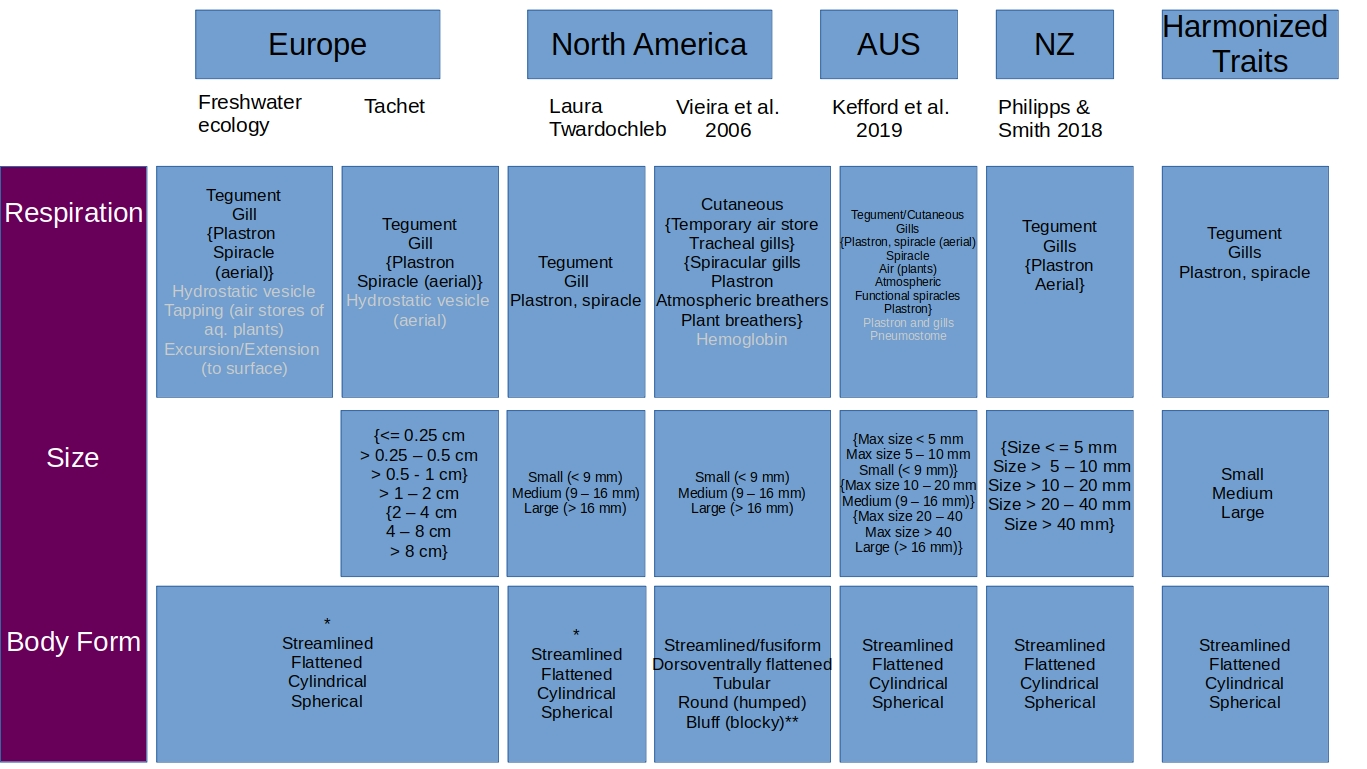
\includegraphics[width=16.5cm, height=10cm]{trait_overview2.jpg}
    \caption{Proposed harmonization scheme for the grouping features
    respiration, size and body form.\newline
    \textit{* Body form information provided by Philippe 
    Usseglio-Polatera.}\newline
    \textit{** Bluff(blocky) taxa have been reclassified
    by Philippe Usseglio-Polatera using the traits streamlined,
    flattened, cylindrical and spherical.} }
    \label{fig:harmon_overview_2}
 \end{figure}

% TODO: Go deeper -> Trait definitions
% !Trait harmonization subjective & always dangerous
Not only the categorization of grouping features but also the definitions of individual traits vary between
databases, complicating harmonization. 
% TODO: Present definition comparison -> For all traits?

\subsection{Aggregation of traits}
% TODO Describing \& testing different approaches
% TODO Problem of coding of traits

%! Description trait aggregation
% ? Aggregation considering different levels of taxonomical resolution
Traits in the processed and harmonized trait databases were aggregated using three approaches.
I) taxa on species-level and genus-level were stepwise aggregated to the family-level by initially 
allocating them at the genus-level using the median. Then all traits were aggregated to family-level by using the mode. 
In cases where it was not possible to take the mode, e.g. only distinct values, multiple duplicates, or multiple 
duplicates and distinct values occurred the mean was taken. Hereafter, we abbreviate this aggregation type as \textit{stepwise\_agg}.
II) we directly aggregated taxa to family level using the median. We denote this aggregation as \textit{direct\_agg}.
III) taxa were aggregated using a weighted approach, denoted as \textit{weighted\_agg}. 
The weights were determined as the ratio of how many taxa on species or genus-level were initially present per genera compared to  
how many taxa on species or genus-level were present after selecting only taxa with complete trait profiles. 
After determining the weights, taxa on species and genus-level were were aggregated to genus-level by multiplying their
trait values by their respective weights. Then the weighted trait values were summed up per family for each trait.

The resulting aggregated trait values were compared to trait values assigned at family-level by experts. 
Trait assignments on family-level existed for the Australian database and the North American database, 
but only for a limited subset of grouping features and taxa. For the Australian database we could
compare aggregated trait values with assigned trait values for the grouping features feeding mode and 
size. For the North American database we compared aggregated trait values with assigned trait values for
the grouping features feeding mode, respiration, size, voltinism and locomotion, 
albeit only for aquatic insects. 
% TODO: Cite Chessman & Matt Pyne
% TODO: At for which traits
% TODO: ATM done with all Taxa, just subset to Species data (does this make sense?)


\section{Results}
% TODO: For Results & Discussion taxonomic overlap between databases rather small

%%%%%%%%%%%%%%%%%%%%%%%%%%%%% MAIN RESULTS %%%%%%%%%%%%%%%%%%%%%%%%%%%%%
% Data preparation complex -> many decisions
% Databases are not ideal (not standardized, different trait definitions)
% Report missing information -> How many families not "get lost"
% Effect of trait aggregation
% Trait values only slightly vary between complex and direct aggregation
 % -> compare with family assignments: Roughly 25 % are classified differently
    % -> Which and why? 
    % -> Add statistical technique -> Maybe clustering?  
 % -> test with weights?
 % -> (effect of transforming binary to fuzzy codes -> US data subset test)
%%%%%%%%%%%%%%%%%%%%%%%%%%%%% MAIN RESULTS %%%%%%%%%%%%%%%%%%%%%%%%%%%%%
%!General overview, how many taxa, distinct orders, ...
\subsection{Taxonomical coverage}
Regarding the taxonomical coverage the New Zealand database has, as expected, the smallest 
taxon pool. In total 492 taxa are covered by this database. Thereof, 404 taxa resolved on species-level, 47 taxa 
on genus-level and 27 taxa on family-level. The remaining entries are on a lower taxonomical resolution. 
73 \% of taxa in the New Zealand database belong to the group of aquatic insects.
The largest taxon pool is spanned by the European trait database, with 4224 taxa of 76 different orders. 
48 \% of the taxa in this database belong to the group of aquatic insects. The European database is 
mostly on the highest taxonomical resolution possible, with 3953 taxa on species-level (approximately 93,6 \%).
253 entries are resolved on genus-level and 18 entries on family-level.
The Australian database has 1404 taxa of 64 orders. 52 \% of the taxa covered are aquatic insects. 
564 taxa are resolved on species-level, 578 on genus-level and 260 on family-level.
The North American trait database contained trait information for 3542 taxa of 42 different orders, 
although 63 \% of the taxa in the database belong to the aquatic insects. 2142 entries are on 
species-level, 1074 on genus-level and 50 on family-level. 

%! How big is the data gap?
\subsection{Completeness of trait information}
The percentage of entries with available information for the individual grouping features in the Australian, European and
North American trait databases varied between 5 \% and 99 \%. By contrast, the New Zealand trait database
contained complete trait information for 99 \% to 100 \% of their entries for the individual grouping features (\ref{tab:trait_coverage}).
The greatest data gap was for the grouping feature body form where information was only present for 7 \% of entries
in the Australian and European database, and 26 \% of entries in the North American database. % TODO: Comment in Draft file for Ralf
Selecting only taxa with complete trait profiles for the six grouping features and resolved at least at 
family-level lead to the omission of many taxa in all databases except for the New Zealand database. 
Out of the 21 orders that the New Zealand database covers, taxa of 20 orders remained after the selection process.
For most orders, all families initially included were also included after selecting taxa with complete trait profiles (table \ref{tab:fam_preproc/fam_init}).
By contrast, in the Australian database, only taxa from five orders (Ephemeroptera, Megaloptera, Odonata, Plecoptera, 
and Trichoptera) remained. Within these five orders, there was none where all families included in the database
contained complete trait profiles. % Clearly the lack of data for body form results in the omission of many taxa
In the North American database, taxa of 18 orders had complete trait profiles, in the European database 9 orders. 

\begin{table}[H]
  \centering
  \caption{How many entries have information for the 
  individual grouping features per database.} 
  \label{tab:trait_coverage}
  \begin{tabular}{llr}
    \hline
  Database & Grouping feature & Trait covered [\%] \\ 
    \hline
  Australia & Body form & 5.00 \\ 
    Australia & Feeding mode & 99.00 \\ 
    Australia & Locomotion & 42.00 \\ 
    Australia & Respiration & 70.00 \\ 
    Australia & Size & 78.00 \\ 
    Australia & Voltinism & 49.00 \\ 
    Europe & Body form & 7.00 \\ 
    Europe & Feeding mode & 65.00 \\ 
    Europe & Locomotion & 33.00 \\ 
    Europe & Respiration & 56.00 \\ 
    Europe & Size & 11.00 \\ 
    Europe & Voltinism & 24.00 \\ 
    New Zealand & Body form & 100.00 \\ 
    New Zealand & Feeding mode & 99.00 \\ 
    New Zealand & Locomotion & 99.00 \\ 
    New Zealand & Respiration & 100.00 \\ 
    New Zealand & Size & 100.00 \\ 
    New Zealand & Voltinism & 100.00 \\ 
    North America & Body form & 26.00 \\ 
    North America & Feeding mode & 61.00 \\ 
    North America & Locomotion & 51.00 \\ 
    North America & Respiration & 44.00 \\ 
    North America & Size & 75.00 \\ 
    North America & Voltinism & 47.00 \\ 
    \hline
  \end{tabular}
  \end{table}

% ?Overview how complete each trait is, by order

% TODO: Mention orders that are not represented at all 
% TODO: Which entries have 0 %, which were not present initially?
% ? Why difference for NOA & NOA_FC? -> rather exclude NOA_FC since it is a special case
\begin{table}[H]
  \centering
  \caption{Proportion of families per order that remain
  after only taxa with complete trait profiles have been selected from the total
  number of distinctive families in the databases.} 
  \label{tab:fam_preproc/fam_init}
  \begin{tabular}{lrrrr}
    \hline
  Order & Australia & New Zealand & Europe & North America \\ 
    \hline
  Amphipoda &  & 100.00 & 37.50 & 10.00 \\ 
    Anthoathecata &  & 100.00 &  &  \\ 
    Architaenioglossa &  &  &  & 100.00 \\ 
    Arhynchobdellida &  &  &  & 100.00 \\ 
    Branchiopoda &  &  &  & 100.00 \\ 
    Coleoptera &  & 88.89 & 83.33 & 15.62 \\ 
    Cycloneritida &  &  &  & 100.00 \\ 
    Decapoda &  & 100.00 &  &  \\ 
    Diptera &  & 100.00 & 46.15 & 21.62 \\ 
    Ephemeroptera & 50.00 & 100.00 & 66.67 & 73.91 \\ 
    Hemiptera &  & 50.00 & 63.64 & 47.06 \\ 
    Hexapoda &  & 100.00 &  &  \\ 
    Lepidoptera &  & 100.00 &  &  \\ 
    Littorinimorpha &  &  &  & 66.67 \\ 
    Mecoptera &  & 100.00 &  &  \\ 
    Megaloptera & 50.00 & 100.00 &  & 50.00 \\ 
    Mollusca &  & 100.00 &  &  \\ 
    Mysida &  & 100.00 &  &  \\ 
    Nemertea &  & 100.00 &  &  \\ 
    Neuroptera &  & 100.00 &  &  \\ 
    Odonata & 6.90 & 100.00 & 100.00 & 50.00 \\ 
    Oligochaeta &  & 100.00 &  &  \\ 
    Onychura &  &  &  & 100.00 \\ 
    Plecoptera & 25.00 & 100.00 & 100.00 & 88.89 \\ 
    Rhynchobdellida &  & 100.00 &  & 50.00 \\ 
    Spinicaudata &  &  &  & 100.00 \\ 
    Tanaidacea &  & 100.00 &  &  \\ 
    Trichoptera & 52.17 & 100.00 & 95.45 & 71.43 \\ 
    Venerida &  &  & 100.00 & 33.33 \\ 
     \hline
  \end{tabular}
  \end{table}

\subsection{Deviance in trait values}
% !How many taxa end up with different trait values after aggregation?(%) 
% TODO: Improve R script
% TODO: Write paragraph
% TODO: Add graphs?
% Generally both methods result in similar values on family-level.
% When deviations, then rather small
% Complex agg: Seems to make only sense with cases where many observations 
% -> many species per Genera, many genera per family

% Deviating cases: mostly Trichoptera, North America Ephemeroptera
% No family that shows deviating results across all databases

% TODO: Comment -> Suggest to Ralf other approaches, if time test them
The \textit{stepwise\_agg} and \textit{direct\_agg} approaches yielded for the majority of taxa 
the same trait values (table \ref{tab:diff_trait_agg_methods}) across all grouping features.  
The two aggregation methods differed the most when applied to the Australian trait database, with 3.52 \% 
cases differently classified. 
% ? How much are trait values deviating?

%! Taxa on family-level that were wrongly classified in all databases


% ! Which traits/grouping features show mainly different values between both aggregation methods?
% in all four databases: feed_herbivore, feed_gatherer, feed_shredder,
% resp_gil, resp_teg, size_medium, size_small result 
\begin{table}[ht]
    \centering
    \caption{Percentage of cases where the \textit{stepwise\_agg} and \textit{direct\_agg} methods 
    resulted in different trait values on family-level.}
    \label{tab:diff_trait_agg_methods}
    \begin{tabular}{lr}
      \hline
    Database & Deviating cases [\%] \\ 
      \hline
    Australia & 3.52 \\ 
      Europe & 2.17 \\ 
      New Zealand & 1.03 \\ 
      North America & 2.66 \\ 
       \hline
    \end{tabular}
    \end{table}

% ! Comparison with traits assigned on family level
% ? Influence on hierarchical clustering

% ! Comparison trait definitions?
% 

%%%%%%%%%%%%%%%%%%%% \section*{Additional ideas} %%%%%%%%%%%%%%%%%%%%

% Section Description of databases:
% \begin{itemize}
%     \item Describe different databases briefly?
%     \item State goal of analysis $\rightarrow$ reference to second paper?
% \end{itemize}

\end{document}